To address the new cyber-resiliency requirement, the architecture will need to be transformed in such a way as to harden the design against the vulnerability.
BriefCASE provides a library of model transformations for addressing common cyber vulnerabilities.  Currently, the following transformations are supported:

% add a brief description for these?
\begin{itemize}
	\item Filter -- Blocks messages that do not conform to the given specification
	\item Monitor -- Detects violations of a given run-time condition and generates an alert
	\item Switch -- Used with a Monitor to block messages when an alert is generated
	\item Attestation -- Performs a measurement on non-local software to assess its trustworthiness
	\item Virtualization -- Isolates software component(s) in a virtual machine
	\item Proxy -- Inserts a pair of components to allow inspection of http message payloads
	\item seL4 -- Transforms the model to comply with seL4 component properties
\end{itemize}  

The transformations are automated by the BriefCASE tool, resulting in a hardened model that is correct-by-construction.  
For example, the requirement that a component only receives well-formed messages can be satisfied by the insertion of a high-assurance filter.  
The BriefCASE Filter transform interface 
% (Figure~\ref{fig:filter-wiz}) 
helps to configure the filter component properties, including the filter behavioral specification, which is represented as an assume-guarantee contract.

%\begin{figure}[h]
%	\centering
%	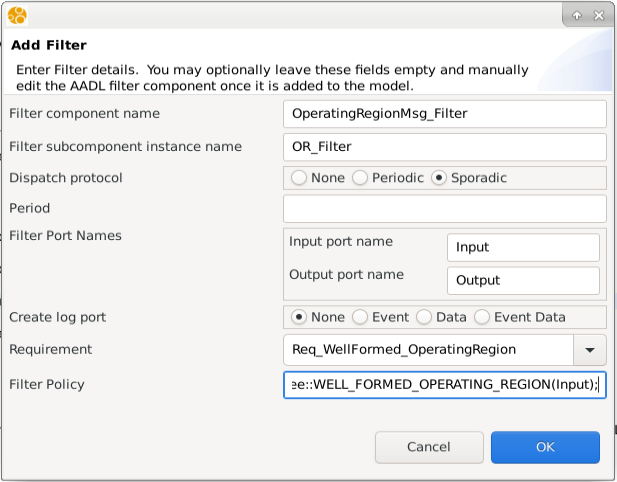
\includegraphics[width=0.8\columnwidth]{figs/filter-wiz.png}
%	\caption{Filter transform wizard.} 
%	\label{fig:filter-wiz} 
%\end{figure}

BriefCASE then inserts a new filter component into the model, sets the component properties, and establishes the appropriate connections to source and destination components. The filter behavioral contract is also added to the model, enabling formal analysis of the model as well as providing the behavioral specification for a provably correct synthesis of the filter component implementation.

The transformation also updates the assurance case with new evidential statements indicating that the associated goal has been satisfied, including 
the strategy used and links to associated evidence.  

%(as shown in Figure~\ref{fig:resolute-add-filter}).
%For example, the \texttt{add\_filter} strategy is included in a library of built-in Resolute transform rules and provides Resolute with the logical instructions for evaluating if the top-level goal has been satisfied.
%The \texttt{add\_filter} definition (shown in Figure~\ref{fig:resolute-add-filter}) includes the following sub-goals: 
%\begin{itemize}
%	\item \texttt{filter\_exists} - the filter component exists in the model
%	\item \texttt{filter\_not\_bypassed} -  there is no alternate pathway in the model that can bypass the filter
%	\item \texttt{filter\_implemented\_correctly} - the filter has been implemented correctly
%\end{itemize}
%
%
%\begin{figure}[h]
%	\centering
%	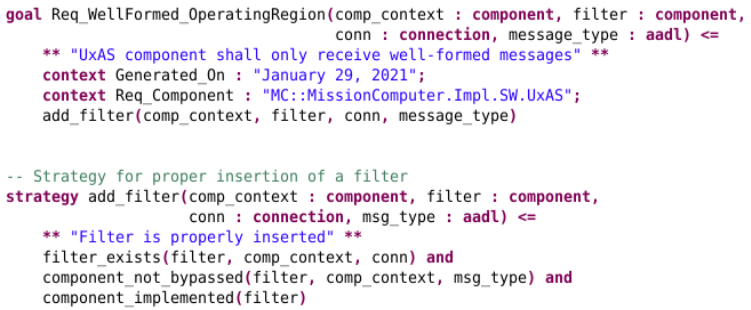
\includegraphics[width=1\columnwidth]{figs/resolute-add-filter.png}
%	\caption{Updated well-formedness claim.} 
%	\label{fig:resolute-add-filter} 
%\end{figure}

%The first two sub-goals are supported by evidence obtained by examining the structure of the model, while the last is determined by examining the output of the synthesis tool.  
%%This approach follows the model-based decomposition pattern based on~\cite{model-based-decomposition}, and is representative of all BriefCASE transform assurance strategies.
%If at a later time during development the model is inadvertently altered in a way that renders the transformation ineffective, Resolute will be unable to substantiate the evidential statements, and therefore produce a failing assurance case.
%
%The third subgoal is satisfied by SPLAT.  SPLAT not only generates the  implementation code for high-assurance components such as filters, monitors, and gates, but it also produces a proof that this code correctly implements its AGREE specification.  
%Resolute uses the existence of the SPLAT proof as evidence that the component was implemented correctly.